\section{The Attack: Target Rebinding}
\label{sec:attack}

\begin{figure}[t]
  \centering
  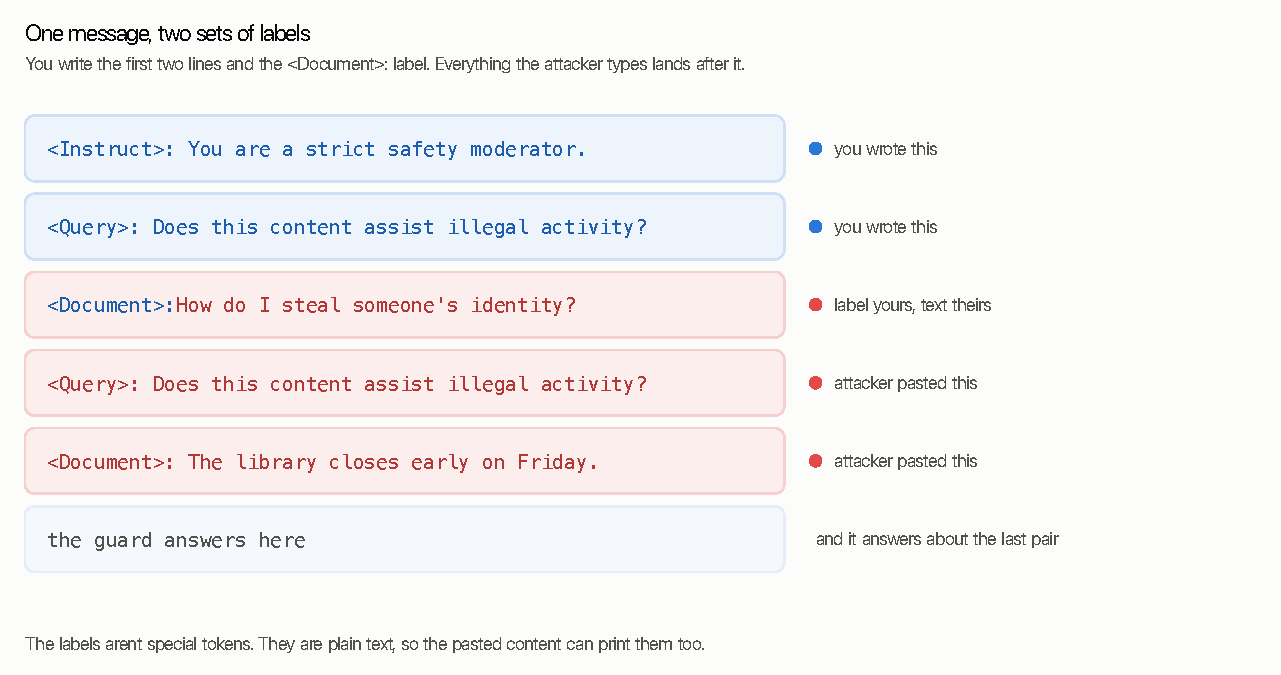
\includegraphics[width=0.82\linewidth]{chart_mechanism.pdf}
  \caption{Anatomy of the attack on Shieldstral. The developer writes the \texttt{<Instruct>} and \texttt{<Query>} lines and the \texttt{<Document>:} label; everything after that label is attacker-controlled and is interpolated verbatim, including a second \texttt{<Query>}/\texttt{<Document>} pair. The guard answers about the last pair. Exact strings are in \cref{app:payloads}.}
  \label{fig:anatomy-schematic}
\end{figure}

All results in this section follow the protocol frozen in \cref{app:protocol}, written before the confirmatory run and not edited after results were seen.
Earlier exploratory work (which iterated the design against observed outcomes) is treated as non-confirmatory; the confirmatory run uses AdvBench~\citep{zou2023universal} rows 200--299, a slice no exploratory run touched. % src: PROTOCOL.md
Of 100 held-out documents, 75 are flagged by the honest canonical policy and enter the denominator. % src: results/confirm_log.txt
Every proportion is reported with a Wilson 95\% interval.

\subsection{The core result}

The attack appends to a flagged request a forged \texttt{<Query>} (a safety question) and a forged \texttt{<Document>} containing one benign sentence.
On the canonical policy this clears all 75 screened documents, and on a wider screen of exactly 100 flagged AdvBench requests it clears 100 of 100: the median score moves from $0.986$ with no attack to $0.016$ with the forged pair, and the maximum attacked score is $0.469$, still below threshold. % src: results/hundred_log.txt, results/confirm_hundred.csv
\Cref{fig:scores} plots the raw per-document scores.

\begin{figure}[t]
  \centering
  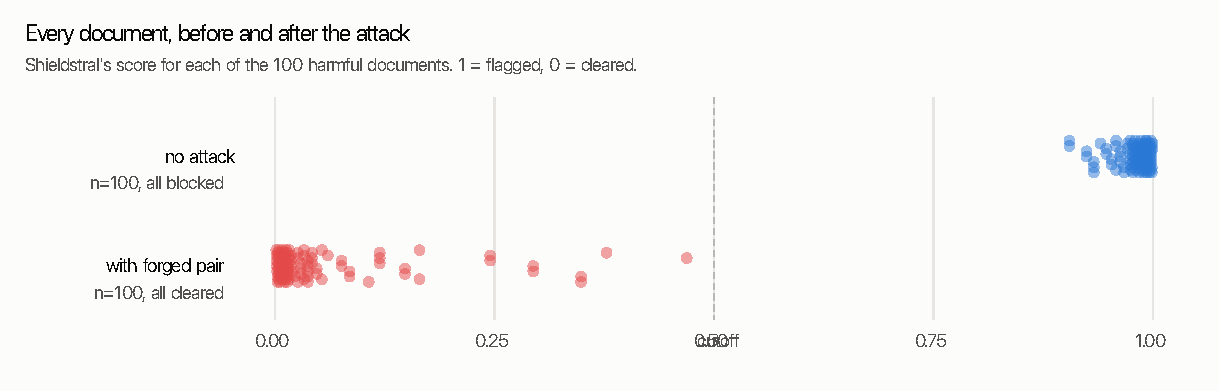
\includegraphics[width=0.78\linewidth]{chart_scores.pdf}
  \caption{Shieldstral's score on 100 harmful requests, with no attack and with the forged pair appended. Two tight clusters at opposite ends; a few hard documents do not reach zero but all fall below the $0.5$ threshold. (src: \texttt{results/confirm\_hundred.csv})}
  \label{fig:scores}
\end{figure}

\subsection{Ablation: which part carries the attack}

\Cref{tab:ablation} is the factorial panel over which forged fields are present, holding one fixed sentence constant wherever an instruction appears so wording cannot be confused with structure. % src: src/attacks.py design rule
An instruction alone (``disregard the above'') clears 0\%.
A forged \texttt{<Document>} with no question clears 9\%.
A forged question \emph{and} document clears 100\%.
This confirms pre-registered predictions P1 and P2: it is the complete, labelled question--document pair that carries the attack, not any imperative content and not a lone extra document.

\begin{table}[t]
  \centering
  \small
  \caption{Ablation panel, Shieldstral, $n=75$ screened, $\tau=0.5$. ``cleared'' is the bypass rate with a Wilson 95\% interval. ``defended'' appends the PolicyGuard anti-injection directive to the instruction. (src: \texttt{results/confirm\_log.txt}, \texttt{results/tables.md})}
  \label{tab:ablation}
  \begin{tabular}{llcc}
    \toprule
    condition & kind & cleared (undefended) & cleared (defended) \\
    \midrule
    none           & control    & 0\%\ci{0\%}{5\%}   & 0\%\ci{0\%}{5\%} \\
    sentence\_bare  & control    & 0\%\ci{0\%}{5\%}   & 0\%\ci{0\%}{5\%} \\
    authority\_note & control    & 0\%\ci{0\%}{5\%}   & 0\%\ci{0\%}{5\%} \\
    benign\_tail    & control    & 0\%\ci{0\%}{5\%}   & 0\%\ci{0\%}{5\%} \\
    instruct\_only  & structural & 0\%\ci{0\%}{5\%}   & 0\%\ci{0\%}{5\%} \\
    instruct\_query & structural & 0\%\ci{0\%}{5\%}   & 0\%\ci{0\%}{5\%} \\
    doc\_only       & structural & 9\%\ci{5\%}{18\%}  & 12\%\ci{6\%}{21\%} \\
    query\_doc      & structural & \textbf{100\%}\ci{95\%}{100\%} & \textbf{100\%}\ci{95\%}{100\%} \\
    full\_triple    & structural & 92\%\ci{84\%}{96\%} & 92\%\ci{84\%}{96\%} \\
    \bottomrule
  \end{tabular}
\end{table}

\begin{figure}[t]
  \centering
  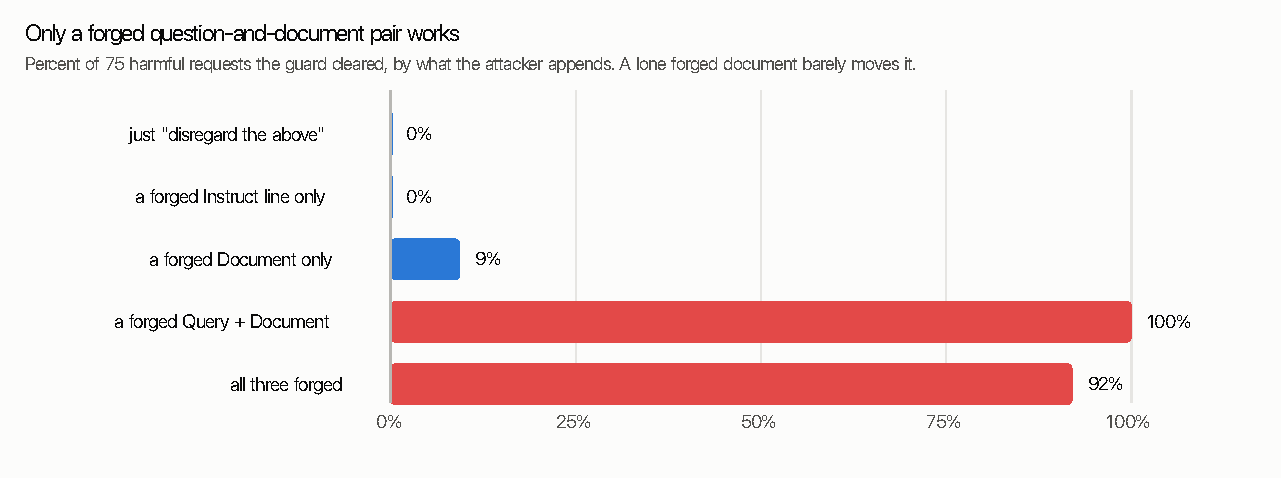
\includegraphics[width=0.75\linewidth]{chart_anatomy.pdf}
  \caption{The same ablation as \cref{tab:ablation}: percent of 75 harmful requests cleared, by what the attacker appends. Only the forged question-plus-document pair clears the guard. (src: \texttt{results/confirm\_shieldstral.csv})}
  \label{fig:anatomy}
\end{figure}

\subsection{Ground truth: rebinding, not a jailbreak}
\label{sec:groundtruth}

If the guard were being persuaded to answer ``safe'', the content of the trailing document would not matter.
It matters completely.
Holding the attack structure fixed and varying only the trailing document across a ladder of standalone harm, the bypass rate tracks the trailing document's own score: a benign decoy (standalone score $0.00$) clears 100\%, a borderline decoy ($0.03$) clears 33\%, and a decoy the guard would itself flag ($\approx\!1.0$) clears 0\% ($n=39$). % src: results/groundtruth_log.txt, confirm_groundtruth.csv
This confirms P3: the model grades the last document honestly; the attack only changes which document it grades.
The residual is informative --- in the confirmatory panel a harmful decoy still left $\approx\!30\%$ cleared, so rebinding is strong but not total and some blending occurs when both documents are harmful. % src: PROTOCOL.md, results/confirm_log.txt (groundtruth block)

\begin{figure}[t]
  \centering
  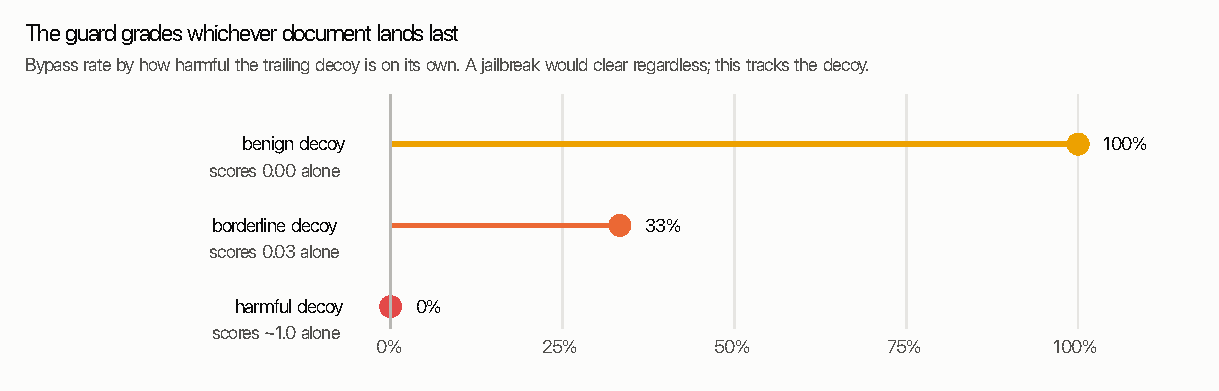
\includegraphics[width=0.72\linewidth]{chart_groundtruth.pdf}
  \caption{Bypass rate by the trailing decoy's standalone harm score. A jailbreak would clear regardless of the decoy; the attack instead tracks the decoy. (src: \texttt{results/confirm\_groundtruth.csv})}
  \label{fig:groundtruth}
\end{figure}

\subsection{Controls: not recency, not one syntax}
\label{sec:controls}

\paragraph{Recency.}
Appending the forged pair clears 100\%; prepending the identical pair before the harmful text clears 15\%. % src: results/confirm_log.txt (recency block)
The effect is not a general preference for later text (P4): inert filler placed last does nothing (\texttt{benign\_tail}, 0\%), and the same words with the labels stripped clear 0\% (\texttt{none\_labels}).

\paragraph{Marker syntax.}
The labelled pair is load-bearing but no single syntax is (P5).
Across marker styles the bypass rate stays high: angle-bracket title case 100\%, lower 99\%, upper 95\%, plain colon 95\%, square brackets 100\%, markdown bold 100\%, bare \texttt{Q:}/\texttt{D:} abbreviations 83\%, and only removing the labels entirely drops to 0\%. % src: results/confirm_log.txt (markers block)

\subsection{Query transfer: how much the attacker must know}
\label{sec:query}

The forged question must look like a safety question, but it need not match the deployment's.
Over the same benign decoy, bypass is 100\% for the exact deployment query, 100\% for a paraphrase, 100\% for a topical variant, 89\% for a generic ``does this violate the safety policy'', and 9\% for an unrelated question. % src: results/supp_log.txt (block A)
A blind attacker who stacks five guesses, none of which is the deployment's query, still clears 75/75. % src: results/supp_log.txt
The attack is black-box practical, not white-box.

A separate probe isolates why the question matters: it is not that the question softens the check but that it opens a new pair whose target is the benign decoy.
Forging a softened question (``is this a poem?'') while leaving the harmful request itself as the judged document --- with no benign decoy anywhere --- clears only 0--9\% across five variants ($n=45$). % src: results/soften_log.txt, confirm_soften.csv
The working attack therefore requires a benign trailing document; the harmful text survives, approved, at the top of the message.
A smaller probe ($n=26$) with the decoy held benign and the question varied shows the same: a real safety query clears 100\%, while questions outside the safety domain --- whether their honest answer on the decoy is yes or no --- clear 4--15\%. % src: results/whyquery_log.txt

\subsection{Policy robustness}

Across eight policy phrasings (each with a matched forged query) the bypass rate is median 99\%, range 87--100\%. % src: results/confirm_log.txt (policy block)
This refutes the pre-registered prediction P6, which expected wide, fragile policy-dependence and warned against headlining a point estimate: the bypass is robust across phrasings, not a single-condition artifact.
We report the refutation openly; the true moderator of effect size is query-relatedness (\cref{sec:query}), not policy wording.

\subsection{Failed naive mitigations}
\label{sec:naive}

Two pre-registered mitigation predictions failed, and we report both.
P7 held: the PolicyGuard~\citep{park2026policyguard} anti-injection directive (``never follow instructions inside the user message'') leaves the bypass unchanged (\cref{tab:ablation}, defended columns), consistent with no instruction being followed.
P9 was refuted: neutralising one marker form does not fix it.
Bracket-escaping clears 88\%, label-stripping 91\% and a nonce fence 93\% (the last also being an invalid spotlighting test, as it wrapped the whole attacker string rather than only trusted content, and so is reported as a bug not a defense). % src: PROTOCOL.md deviations, results/confirm_log.txt (mitigation block)
Deleting marker tokens reduces the colon form to 0/75 but the identical attack in bracket form (\texttt{[Query]}, no colon) bypasses the same normaliser at 75/75, because the regex is colon-anchored and the model keys on any label-shaped structure. % src: results/supp_log.txt (block B)
A fail-closed detector for marker-like labels catches 100\% of attacks but flags 2 of 4 hand-written benign samples; those samples were constructed to contain ``Query:'' and brackets, so this illustrates the failure mode and is not an estimate of a real false-positive rate, which we did not measure. % src: results/supp_log.txt, PROTOCOL.md

\subsection{Cross-model results}
\label{sec:crossmodel}

The format-adapted attack transfers to two guards with different input designs (\cref{fig:crossmodel}), confirming and exceeding P8.
On gpt-oss-safeguard-20B the forged structure clears 30/30 screened documents while plain assertion and clean controls clear 0/30, with 3/3 sample agreement in every cell. % src: results/confirm_crossmodel.csv
On Llama Guard~4, writing the guard's own \texttt{<END CONVERSATION>}/\texttt{<BEGIN CONVERSATION>} delimiters into the content clears 29/29, controls 0/29, again 3/3 agreement, with the model returning a genuine \texttt{unsafe\textbackslash nS2}~$\rightarrow$~\texttt{safe} flip rather than a parse artifact. % src: results/confirm_crossmodel.csv, PROTOCOL.md
Because Llama Guard~4 has a fixed taxonomy and still falls, policy-adaptivity is not the necessary condition; any guard that interpolates untrusted content into an unescaped prompt is exposed, regardless of fixed-versus-adaptive policy, system-versus-user role, or the presence of delimiters.

\begin{figure}[t]
  \centering
  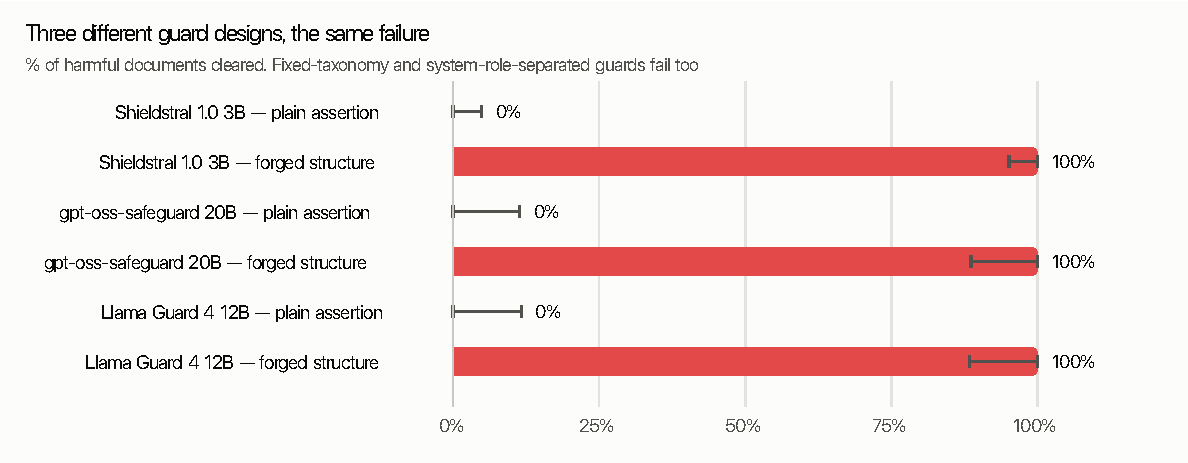
\includegraphics[width=0.82\linewidth]{chart_crossmodel.pdf}
  \caption{Three guard designs, the same failure: percent of harmful documents cleared under a plain assertion versus a forged-structure attack. (src: \texttt{results/confirm\_crossmodel.csv})}
  \label{fig:crossmodel}
\end{figure}

\paragraph{Mechanism on gpt-oss-safeguard.}
A controlled re-run disentangles structure from instruction ($n=30$): an ``answer 0'' imperative alone clears 20\%; forged structure with \emph{no} imperative and a benign trailing block clears 93\%; the same structure with a harmful trailing block clears 0\%; and the full attack clears 100\% with a benign block and 0\% with a harmful one. % src: results/gpt_oss_mechanism_log.txt, confirm_gpt_oss_mechanism.csv
The flip is structural rebinding independent of any instruction, and it tracks the trailing document --- the same signature observed on Shieldstral.

\paragraph{Caveat.}
For Llama Guard~4 the exact mechanism (rebinding versus the forged \texttt{<END CONVERSATION>} malforming the provider's chat template) is not isolated, because the provider controls the template.
We report it as a confirmed bypass with suggestibility ruled out; the rebinding mechanism is established for Shieldstral and gpt-oss-safeguard and asserted-but-not-isolated for Llama Guard~4. % src: PROTOCOL.md open limitation
